\chapter{HỆ THỐNG EASYMESH}
\label{chapter:chapter-2}
% ============================================================
\section{Tổng quan Hệ thống Wi-Fi Mesh}
% ============================================================

Hệ thống Wi-Fi Mesh là giải pháp mở rộng vùng phủ sóng Wi-Fi bằng cách kết nối nhiều
điểm truy cập (Access Point --- AP) thành một mạng lưới thống nhất. Thay vì người dùng
phải cấu hình riêng từng AP, toàn bộ hệ thống hoạt động dưới \textbf{một tên mạng
	(SSID) duy nhất} và thiết bị khách (STA) được tự động chuyển vùng giữa các AP mà
không cần ngắt kết nối. Các thành phần trong mạng Wi-Fi Mesh được mô tả trên hình
\ref{fig:EasyMeshSystemModel}, bao gồm:

\begin{enumerate}
	\item \textbf{Controller:} AP đảm nhận vai trò trung tâm điều phối toàn mạng Mesh.
	Controller là điểm kết nối ra Internet (gateway), là nơi lưu trữ duy nhất các
	cấu hình Wi-Fi của toàn mạng (SSID, mật khẩu, chính sách) và đồng bộ chúng
	xuống tất cả Agent thông qua chuẩn IEEE~1905.1.
	
	\item \textbf{Agent:} AP đảm nhận vai trò mở rộng vùng phủ. Agent nhận cấu hình
	từ Controller, phát sóng Wi-Fi cho thiết bị người dùng (qua fBSS) và duy trì
	liên kết Backhaul lên Controller hoặc Agent cha (qua bSTA). Một mạng Mesh có
	thể có nhiều Agent kết nối nối tiếp nhau thành chuỗi (Daisy Chain) hoặc hình
	sao (Star).
	
	\item \textbf{AL MAC (Abstraction Layer MAC):} Địa chỉ định danh duy nhất của mỗi
	thiết bị trong mạng Mesh theo chuẩn IEEE~1905.1. Tất cả bản tin điều khiển
	1905 dùng AL MAC làm địa chỉ nguồn và địa chỉ đích. Đối với bản tin
	Multicast, địa chỉ đích quy định là \texttt{01:80:C2:00:00:13}.
	
	\item \textbf{fBSS (Fronthaul BSS):} BSS phát sóng trên AP (Controller hoặc Agent)
	để các thiết bị người dùng (STA) kết nối vào. Đây là mạng Wi-Fi mà người
	dùng cuối nhìn thấy và sử dụng hàng ngày.
	
	\item \textbf{bBSS (Backhaul BSS):} BSS phát sóng trên Controller hoặc Agent cha,
	chuyên dành cho các Agent con (bSTA) kết nối Backhaul lên. bBSS không hiển
	thị với thiết bị người dùng thông thường.
	
	\item \textbf{bSTA (Backhaul STA):} Giao diện Wi-Fi trên Agent dùng để kết nối lên
	bBSS của Controller hoặc Agent cha, thiết lập liên kết Backhaul không dây
	giữa các AP trong mạng Mesh.
\end{enumerate}

% ================================================================
% Hình 1: EasyMeshSystemModel.png
% ================================================================
\begin{figure}[ht]
	\centering
	\begin{tikzpicture}[>=stealth, font=\small]
		
		% ---- Vùng phủ sóng ----
		% Controller (tâm: -2, 0)
		\draw[yellow!70!orange, dotted,  line width=1.4pt] (-2.0, 0.0) circle (4.0cm);
		\draw[pink!80!red,      dashed,  line width=1.4pt] (-2.0, 0.0) circle (2.9cm);
		% Agent 1 (tâm: 3.5, 2.5)
		\draw[yellow!70!orange, dotted,  line width=1.4pt] (3.5,  2.5) circle (3.0cm);
		\draw[pink!80!red,      dashed,  line width=1.4pt] (3.5,  2.5) circle (2.2cm);
		% Agent 2 (tâm: 3.0, -2.5)
		\draw[yellow!70!orange, dotted,  line width=1.4pt] (3.0, -2.5) circle (3.0cm);
		\draw[pink!80!red,      dashed,  line width=1.4pt] (3.0, -2.5) circle (2.2cm);
		
		% ---- Internet cloud ----
		\node[cloud, draw, thick, cloud puffs=9, cloud puff arc=110,
		minimum width=2.4cm, minimum height=1.4cm, fill=white]
		(cloud) at (-6.5, 0) {\small Internet};
		
		% ---- Ethernet Cable: Internet → Controller ----
		\draw[very thick] (-5.3, 0) -- (-2.6, 0);
		\node[above, scale=0.70] at (-3.95, 0.08) {Ethernet Cable};
		
		% ---- Icon: Controller ----
		\draw[thick, fill=gray!25, rounded corners=2pt]
		(-2.55,-0.25) rectangle (-1.45, 0.25);
		\draw[thick] (-2.22, 0.25) -- (-2.32, 0.68);  % anten trái
		\draw[thick] (-1.78, 0.25) -- (-1.68, 0.68);  % anten phải
		\node[below, scale=0.75, font=\bfseries] at (-2.0,-0.30) {Controller};
		
		% ---- Backhaul Wi-Fi: Controller → Agent 1 (hồng) ----
		\draw[pink!80!red, line width=2.5pt]
		(-1.45, 0.15)
		-- (-0.28, 0.65) -- (-0.56, 1.15)
		-- ( 0.90, 1.62) -- ( 0.62, 2.04)
		-- ( 2.10, 2.34) -- ( 3.05, 2.48);
		\node[pink!65!red, rotate=23, scale=0.70] at (0.82, 1.56) {Wi-Fi};
		
		% ---- Backhaul Wi-Fi: Controller → Agent 2 (hồng) ----
		\draw[pink!80!red, line width=2.5pt]
		(-1.45,-0.15)
		-- (-0.28,-0.75) -- (-0.56,-1.15)
		-- ( 0.85,-1.68) -- ( 0.55,-2.08)
		-- ( 1.95,-2.33) -- ( 2.55,-2.48);
		\node[pink!65!red, rotate=-26, scale=0.70] at (0.80,-1.68) {Wi-Fi};
		
		% ---- Icon: Agent 1 ----
		\draw[thick, fill=gray!25, rounded corners=2pt]
		(3.05, 2.22) rectangle (3.95, 2.72);
		\draw[thick] (3.30, 2.72) -- (3.18, 3.15);
		\draw[thick] (3.70, 2.72) -- (3.82, 3.15);
		\node[below, scale=0.75, font=\bfseries] at (3.5, 2.18) {Agent 1};
		
		% ---- Fronthaul Wi-Fi: Agent 1 → STA (vàng) ----
		\draw[yellow!65!orange, line width=2.0pt]
		(3.95, 2.58)
		-- (4.72, 2.78) -- (4.50, 3.10)
		-- (5.28, 3.22) -- (5.05, 3.54)
		-- (5.90, 3.60);
		\node[yellow!55!orange, scale=0.70] at (5.08, 3.05) {Wi-Fi};
		
		% ---- Icon: STA (điện thoại) ----
		\draw[thick, rounded corners=3pt, fill=cyan!20]
		(5.90, 3.08) rectangle (6.60, 4.10);
		\draw[thick] (6.10, 3.16) -- (6.40, 3.16);
		\node[below, scale=0.68] at (6.25, 3.08) {STA};
		
		% ---- Icon: Agent 2 ----
		\draw[thick, fill=gray!25, rounded corners=2pt]
		(2.55,-2.72) rectangle (3.45,-2.22);
		\draw[thick] (2.80,-2.22) -- (2.68,-1.79);
		\draw[thick] (3.20,-2.22) -- (3.32,-1.79);
		\node[below, scale=0.75, font=\bfseries] at (3.0,-2.75) {Agent 2};
		
		% ---- Ethernet: Agent 2 → Laptop ----
		\draw[very thick] (2.78,-2.72) -- (2.08,-3.55);
		\node[right, scale=0.68] at (2.20,-3.15) {Ethernet};
		
		% ---- Icon: Laptop ----
		\draw[thick, fill=gray!15]
		(0.80,-4.15) rectangle (2.65,-3.52);   % màn hình
		\draw[thick, fill=gray!25]
		(0.60,-4.40) -- (0.80,-4.15) --
		(2.65,-4.15) -- (2.85,-4.40) -- cycle; % đế
		\node[below, scale=0.68] at (1.72,-4.42) {Laptop};
		
		% ---- Chú thích ----
		\begin{scope}[shift={(5.5,-0.8)}]
			\node[anchor=west, scale=0.72, font=\bfseries] at (0, 0.35) {Chú thích:};
			\draw[yellow!70!orange, dotted, line width=1.4pt] (0,-0.20) -- (1.10,-0.20);
			\node[anchor=west, scale=0.68] at (1.15,-0.20) {bSTA / fBSS};
			\draw[pink!80!red, dashed, line width=1.4pt] (0,-0.68) -- (1.10,-0.68);
			\node[anchor=west, scale=0.68] at (1.15,-0.68) {bBSS};
			\draw[pink!80!red, line width=2.5pt] (0,-1.16) -- (1.10,-1.16);
			\node[anchor=west, scale=0.68] at (1.15,-1.16) {Backhaul Wi-Fi};
			\draw[yellow!65!orange, line width=2.0pt] (0,-1.64) -- (1.10,-1.64);
			\node[anchor=west, scale=0.68] at (1.15,-1.64) {Fronthaul Wi-Fi};
		\end{scope}
		
	\end{tikzpicture}
	\caption{Mô hình một mạng Wi-Fi Mesh.}
	\label{fig:EasyMeshSystemModel}
\end{figure}

Trên hình \ref{fig:EasyMeshSystemModel}, các \textbf{bSTA} được biểu diễn bằng hình
tròn viền nét đứt màu vàng, \textbf{bBSS} bằng hình tròn viền nét đứt màu hồng. Liên
kết Backhaul giữa bSTA của Agent và bBSS của Controller được tô màu hồng; liên kết
Fronthaul giữa STA người dùng và fBSS trên AP được tô màu vàng.


% ------------------------------------------------------------
\subsection{Triển khai Thực tế Hệ thống Wi-Fi Mesh của VHT}
% ------------------------------------------------------------

Tính đến tháng 12/2024, hệ thống Wi-Fi Mesh của VHT đã được triển khai trên
\textbf{64 tỉnh thành} trên cả nước, với hai dòng thiết bị chính là ONT và AP hỗ trợ
Wi-Fi~5 (802.11ac) và Wi-Fi~6 (802.11ax). Thực tế triển khai bao gồm cả cấu hình
đồng thế hệ lẫn xuyên thế hệ:

\begin{enumerate}
	\item \textbf{ONTw5 -- APw5:} Controller Wi-Fi~5 + Agent Wi-Fi~5 --- cùng thế hệ,
	tham số RF tương thích hoàn toàn.
	\item \textbf{ONTw5 -- APw6:} Controller Wi-Fi~5 + Agent Wi-Fi~6 --- xuyên thế hệ,
	cần lưu ý sự khác biệt về tốc độ kết nối vật lý và băng thông kênh.
	\item \textbf{ONTw6 -- APw6:} Controller Wi-Fi~6 + Agent Wi-Fi~6 --- cùng thế hệ,
	khai thác đầy đủ tính năng MU-MIMO, OFDMA của Wi-Fi~6.
\end{enumerate}

Mesh giữa các thiết bị \textbf{cùng thế hệ} Wi-Fi cho kết quả ổn định hơn nhờ các
tham số RF tương thích. Mesh \textbf{xuyên thế hệ} (Wi-Fi~5 với Wi-Fi~6) đòi hỏi sự
chú ý đặc biệt vì sự khác biệt về tốc độ kết nối vật lý (PHY rate) và băng thông kênh
(Wi-Fi~5 tối đa 160\,MHz, Wi-Fi~6 hỗ trợ đầy đủ 160\,MHz với nhiều cải tiến) có thể
ảnh hưởng đến các thông số tính toán nội bộ của hệ thống, gây lỗi đồng bộ nếu không
được xử lý đúng cách.


% ============================================================
\section{Các Chức năng của Hệ thống Wi-Fi Mesh}
% ============================================================

% ------------------------------------------------------------
\subsection{Đồng bộ Cấu hình (Autoconfiguration)}
% ------------------------------------------------------------

Đây là chức năng nền tảng của mạng Mesh: đảm bảo mọi Agent trong mạng đều nhận và
áp dụng đúng cấu hình Wi-Fi từ Controller --- SSID, mật khẩu, kiểu mã hóa, và vai trò
BSS. Quá trình bắt đầu ngay sau khi Agent thiết lập được kết nối vật lý với mạng
(qua Wi-Fi Backhaul hoặc Ethernet), và được thực hiện qua bốn bản tin theo chuẩn
IEEE~1905.1 mở rộng:

\begin{figure}[ht]
	\centering
	\begin{tikzpicture}[>=stealth, font=\small]
		% --- Tiêu đề ---
		\node[draw, fill=gray!15, minimum width=3cm, minimum height=0.6cm]
		(A) at (0, 0) {Enrollee (Agent)};
		\node[draw, fill=gray!15, minimum width=3cm, minimum height=0.6cm]
		(C) at (9, 0) {Registrar (Controller)};
		
		% --- Lifelines ---
		\draw[dashed, gray!50] (0,-0.4) -- (0,-11.5);
		\draw[dashed, gray!50] (9,-0.4) -- (9,-11.5);
		
		% Bước 1: Autoconfig Search
		\draw[->] (0,-1.4) -- (9,-1.4)
		node[midway, above, scale=0.7, fill=white, inner sep=1pt]
		{(1) Autoconfig Search [Multicast: 01:80:C2:00:00:13]};
		\node[scale=0.6, gray, align=center] at (4.5,-2.1)
		{\textit{Agent phát quảng bá tìm Controller; gửi lại nếu không có phản hồi}};
		
		% Bước 2: Autoconfig Response
		\draw[->] (9,-3.1) -- (0,-3.1)
		node[midway, above, scale=0.7, fill=white, inner sep=1pt]
		{(2) Autoconfig Response};
		\node[scale=0.6, gray, align=center] at (4.5,-3.8)
		{\textit{Controller xác nhận vai trò; Agent chuyển sang bước trao đổi M1/M2}};
		
		% Phân tách pha
		\draw[dashed, gray!60] (-1.5,-4.5) -- (10.5,-4.5);
		\node[scale=0.65, gray!80] at (4.5,-4.85)
		{Lặp lại cho từng băng tần (2.4\,GHz, 5\,GHz, 6\,GHz)};
		
		% Bước 3: M1
		\draw[->, blue] (0,-5.8) -- (9,-5.8)
		node[midway, above, scale=0.7, fill=white, inner sep=1pt]
		{(3) Autoconfig M1 [Public Key, Nonce, Radio Capabilities]};
		\node[scale=0.6, gray, align=center] at (4.5,-6.5)
		{\textit{Agent khai báo khả năng Wi-Fi của từng radio (băng tần, chuẩn, mã hóa hỗ trợ)}};
		
		% Bước 4: M2
		\draw[->, blue] (9,-7.7) -- (0,-7.7)
		node[midway, above, scale=0.7, fill=white, inner sep=1pt]
		{(4) Autoconfig M2 [Encrypted Settings: SSID, PSK, BSS Role]};
		\node[scale=0.6, gray, align=center] at (4.5,-8.4)
		{\textit{Controller gửi cấu hình Wi-Fi mã hóa (SSID, mật khẩu, kiểu xác thực, vai trò BSS)}};
		
		% Bước 5: Agent áp dụng
		\node[draw, dashed, fill=green!8, scale=0.7, align=center] at (0,-9.5)
		{Áp dụng cấu hình\\xuống Driver Wi-Fi};
		
		% Bước 6: Topology Response
		\draw[->, brown] (0,-10.8) -- (9,-10.8)
		node[midway, above, scale=0.7, fill=white, inner sep=1pt]
		{(5) Topology Response [AP Operational BSS TLV]};
		\node[scale=0.6, gray, align=center] at (4.5,-11.4)
		{\textit{Agent xác nhận BSSID thực tế đang hoạt động; Controller cập nhật bản đồ mạng}};
	\end{tikzpicture}
	\caption{Luồng bản tin đồng bộ cấu hình Autoconfig trong IEEE~1905.1 / EasyMesh.}
	\label{fig:autoconfig-flow}
\end{figure}

\begin{enumerate}
	\item \textbf{Autoconfig Search:} Agent phát Multicast lên toàn mạng để tìm
	Controller. Bản tin được chuyển tiếp bởi các Agent trung gian và chỉ được
	phản hồi bởi duy nhất Controller. Nếu không có phản hồi sau thời gian chờ
	định trước, Agent tự động gửi lại (số lần và khoảng cách tùy thiết kế phần
	mềm).
	
	\item \textbf{Autoconfig Response:} Controller phản hồi xác nhận vai trò Registrar
	và cung cấp thông tin cần thiết để Agent thực hiện bước trao đổi M1/M2 tiếp
	theo. Mỗi cặp Search/Response có cùng Message~ID --- bản tin khác ID bị hủy
	bỏ để tránh nhầm lẫn.
	
	\item \textbf{Autoconfig M1:} Agent gửi thông tin khả năng radio: Public Key (trao
	đổi khóa Diffie-Hellman), Nonce (chống replay attack), và chi tiết các chuẩn
	Wi-Fi, phương thức xác thực/mã hóa mà radio đó hỗ trợ. Controller dùng thông
	tin này để lựa chọn cấu hình phù hợp nhất với phần cứng Agent.
	
	\item \textbf{Autoconfig M2:} Controller gửi lại cấu hình Wi-Fi được mã hóa bằng
	khóa đã trao đổi ở M1: SSID, mật khẩu (PSK), kiểu mã hóa và vai trò BSS
	(Fronthaul/Backhaul). Với hệ thống 2 băng tần (2.4\,GHz và 5\,GHz) sẽ có
	\textbf{2 cặp M1/M2} riêng biệt cho từng radio.
\end{enumerate}


\begin{table}[ht]
	\centering
	\caption{Các trường chính trong bản tin M1 (WPS/EasyMesh Autoconfig)}
	\begin{tabular}{|>{\raggedright\arraybackslash}m{4cm}|>{\raggedright\arraybackslash}m{9cm}|}
		\hline
		\textbf{Trường (Field)} & \textbf{Mô tả} \\
		\hline
		Version & Phiên bản WPS, thường là \texttt{0x10} (WPS v1.0) \\
		\hline
		Message Type & Mã xác định bản tin là M1 (\texttt{value = 0x04}) \\
		\hline
		UUID-E & UUID của Enrollee (Agent) --- định danh duy nhất thiết bị \\
		\hline
		Public Key & Khóa công khai của Agent, dùng trao đổi khóa Diffie-Hellman \\
		\hline
		Registrar Nonce & Số ngẫu nhiên do Agent tạo ra, dùng để chống replay attack \\
		\hline
		Authentication Type Flags & Các phương thức xác thực Agent hỗ trợ (WPA2-PSK, WPA3-SAE, \ldots) \\
		\hline
		Encryption Type Flags & Các thuật toán mã hóa hỗ trợ (AES, TKIP, \ldots) \\
		\hline
		Configuration Methods & Phương pháp cấu hình hỗ trợ (Push Button, PIN, \ldots) \\
		\hline
		Connection Type Flags & Loại kết nối (băng tần 2.4\,GHz, 5\,GHz, 6\,GHz) \\
		\hline
		Manufacturer / Model / Serial & Thông tin nhận dạng phần cứng thiết bị Agent \\
		\hline
		Primary Device Type & Loại thiết bị (Access Point) \\
		\hline
		Device Name & Tên hiển thị của thiết bị (dùng trong giao diện quản lý) \\
		\hline
	\end{tabular}
\end{table}

\begin{table}[ht]
	\centering
	\caption{Các trường chính trong bản tin M2 (WPS/EasyMesh Autoconfig)}
	\begin{tabular}{|>{\raggedright\arraybackslash}m{4cm}|>{\raggedright\arraybackslash}m{9cm}|}
		\hline
		\textbf{Trường (Field)} & \textbf{Mô tả} \\
		\hline
		Version & Phiên bản WPS, thường là \texttt{0x10} (WPS v1.0) \\
		\hline
		Message Type & Mã xác định bản tin là M2 (\texttt{value = 0x05}) \\
		\hline
		Enrollee Nonce & Số nonce lấy từ M1 của Agent, để khớp cặp bản tin \\
		\hline
		Public Key & Khóa công khai của Controller, hoàn tất trao đổi Diffie-Hellman \\
		\hline
		Authentication Type Flags & Phương thức xác thực Controller lựa chọn cho Agent \\
		\hline
		Encryption Type Flags & Thuật toán mã hóa được chọn \\
		\hline
		Encrypted Settings & \textbf{Trường quan trọng nhất:} chứa SSID, PSK (mật khẩu), kiểu mã hóa và vai trò BSS (Fronthaul/Backhaul) được mã hóa bằng khóa phiên đã trao đổi \\
		\hline
		Manufacturer / Model / Serial & Thông tin nhận dạng của Controller \\
		\hline
	\end{tabular}
\end{table}


% ------------------------------------------------------------
\subsection{Quản lý Thiết bị (Device Management)}
% ------------------------------------------------------------

Sau khi đồng bộ cấu hình, Controller cần duy trì bức tranh toàn diện về trạng thái
mạng: có bao nhiêu AP, chúng kết nối với nhau như thế nào, và STA nào đang kết nối
vào BSS nào. Thông tin này là nền tảng cho các quyết định điều phối chuyển vùng và
tối ưu hóa Backhaul.

Việc xây dựng và duy trì bản đồ mạng dựa trên bộ bản tin \textbf{Topology} theo
chuẩn IEEE~1905.1, như mô tả trên hình \ref{fig:topology-flow}:

\begin{figure}[ht]
	\centering
	\begin{tikzpicture}[>=stealth, font=\small]
		% --- Tiêu đề ---
		\node[draw, fill=gray!15, minimum width=2.2cm, minimum height=0.6cm]
		(A) at (0,   0) {Device A};
		\node[draw, fill=gray!15, minimum width=2.2cm, minimum height=0.6cm]
		(B) at (5.5, 0) {Device B};
		\node[draw, fill=gray!15, minimum width=2.2cm, minimum height=0.6cm]
		(C) at (11,  0) {Device C};
		
		% --- Lifelines ---
		\draw[dashed, gray!50] (0,  -0.4) -- (0,  -11.5);
		\draw[dashed, gray!50] (5.5,-0.4) -- (5.5,-11.5);
		\draw[dashed, gray!50] (11, -0.4) -- (11, -11.5);
		
		% Phân tách pha 1
		\node[scale=0.72, font=\bfseries, anchor=west] at (-0.5,-1.0)
		{Giai đoạn 1: Khám phá lân cận (Topology Discovery --- Multicast)};
		\draw[gray!60] (-0.5,-1.35) -- (12,-1.35);
		
		\draw[->] (0,-2.1) -- (5.5,-2.1)
		node[midway, above, scale=0.65, fill=white, inner sep=1pt]
		{(1) Topology Discovery [AL MAC, Device Info]};
		\draw[->] (5.5,-3.0) -- (0,-3.0)
		node[midway, above, scale=0.65, fill=white, inner sep=1pt]
		{(2) Topology Discovery [AL MAC, Device Info]};
		\draw[->] (5.5,-3.9) -- (11,-3.9)
		node[midway, above, scale=0.65, fill=white, inner sep=1pt]
		{(3) Topology Discovery [AL MAC, Device Info]};
		\draw[->] (11,-4.8) -- (5.5,-4.8)
		node[midway, above, scale=0.65, fill=white, inner sep=1pt]
		{(4) Topology Discovery [AL MAC, Device Info]};
		
		% Phân tách pha 2
		\node[scale=0.72, font=\bfseries, anchor=west] at (-0.5,-5.8)
		{Giai đoạn 2: Truy vấn chi tiết (Topology Query/Response --- Unicast)};
		\draw[gray!60] (-0.5,-6.15) -- (12,-6.15);
		
		\draw[->] (0,-7.0) -- (5.5,-7.0)
		node[midway, above, scale=0.65, fill=white, inner sep=1pt]
		{(5) Topology Query};
		\draw[->] (5.5,-8.0) -- (0,-8.0)
		node[midway, above, scale=0.65, fill=white, inner sep=1pt]
		{(6) Topology Response [BSS Info, Client List, Link Metrics]};
		
		% Phân tách pha 3
		\node[scale=0.72, font=\bfseries, anchor=west] at (-0.5,-9.0)
		{Giai đoạn 3: Thông báo thay đổi (Topology Notification --- tức thì)};
		\draw[gray!60] (-0.5,-9.35) -- (12,-9.35);
		
		\draw[->, dashed] (0,-10.2) -- (5.5,-10.2)
		node[midway, above, scale=0.65, fill=white, inner sep=1pt]
		{(7) Topology Notification [Client Join/Leave]};
		\node[scale=0.6, gray] at (5.5,-10.95)
		{\textit{Gửi ngay khi có STA kết nối hoặc ngắt kết nối}};
	\end{tikzpicture}
	\caption{Sơ đồ luồng bản tin Topology trong IEEE~1905.1.}
	\label{fig:topology-flow}
\end{figure}

\begin{enumerate}
	\item \textbf{Topology Discovery:} Bản tin Multicast được mỗi thiết bị gửi ra tất
	cả interface ngay khi có kết nối vật lý mới và theo chu kỳ định kỳ (thường
	mỗi 60 giây). Mục tiêu là giúp các thiết bị lân cận phát hiện sự hiện diện
	của nhau và cập nhật thông tin cơ bản (AL~MAC, loại interface).
	
	\item \textbf{Topology Query:} Khi nhận được Discovery từ thiết bị lân cận, AP
	gửi Query Unicast đến thiết bị đó để yêu cầu thông tin chi tiết hơn. Cặp
	Query/Response dùng cùng Message~ID --- bản tin khác ID bị loại bỏ.
	
	\item \textbf{Topology Response:} Phản hồi đầy đủ thông tin về AP: danh sách BSS,
	các STA đang kết nối và thông tin liên kết. Lưu ý: thông tin radio (kênh,
	công suất) \textit{không} nằm trong bản tin này mà được cập nhật riêng qua
	\textbf{Channel Report}; thông số chất lượng liên kết (RSSI, throughput) cập
	nhật qua \textbf{Link Metrics}.
	
	\item \textbf{Topology Notification} (tùy chọn): Gửi \textit{ngay lập tức} khi có
	thay đổi quan trọng (STA kết nối/ngắt kết nối, BSS thay đổi trạng thái) ---
	không chờ chu kỳ Discovery định kỳ, đảm bảo Controller luôn có thông tin
	mới nhất.
\end{enumerate}

\begin{table}[ht]
	\centering
	\caption{Nội dung bản tin Topology Discovery trong IEEE~1905.1}
	\begin{tabular}{|>{\raggedright\arraybackslash}m{5cm}|>{\raggedright\arraybackslash}m{8cm}|}
		\hline
		\textbf{TLV} & \textbf{Mô tả} \\
		\hline
		AL MAC Address TLV & Địa chỉ AL MAC của thiết bị gửi --- định danh duy nhất trong mạng 1905 \\
		\hline
		Device Information TLV & Loại thiết bị, danh sách interface vật lý và trạng thái hoạt động \\
		\hline
		Transmitter Link Metric TLV & Thông số liên kết truyền đi: throughput ước tính, tỉ lệ lỗi \\
		\hline
		Receiver Link Metric TLV & Thông số liên kết nhận về: RSSI, tỉ lệ lỗi \\
		\hline
		IPv4/IPv6 TLV (tùy chọn) & Địa chỉ IP của thiết bị (nếu hỗ trợ) \\
		\hline
		Vendor Specific TLV (tùy chọn) & Thông tin mở rộng theo nhà sản xuất \\
		\hline
	\end{tabular}
\end{table}

\begin{table}[ht]
	\centering
	\caption{Nội dung bản tin Topology Response trong IEEE~1905.1}
	\begin{tabular}{|>{\raggedright\arraybackslash}m{5cm}|>{\raggedright\arraybackslash}m{8cm}|}
		\hline
		\textbf{TLV} & \textbf{Mô tả} \\
		\hline
		AL MAC Address TLV & Địa chỉ AL MAC của thiết bị phản hồi \\
		\hline
		Device Information TLV & Thông tin thiết bị: loại, trạng thái, danh sách interface \\
		\hline
		Transmitter / Receiver Link Metric TLV & Chất lượng các liên kết vật lý (Tx và Rx) \\
		\hline
		IPv4/IPv6 TLV (tùy chọn) & Địa chỉ IP của thiết bị \\
		\hline
		Bridge Discovery TLV (nếu có) & Thông tin về khả năng bridge của thiết bị \\
		\hline
		Vendor Specific TLV (tùy chọn) & Dữ liệu mở rộng theo nhà sản xuất \\
		\hline
	\end{tabular}
\end{table}


% ------------------------------------------------------------
\subsection{Chuyển vùng cho STA (Client Steering)}
% ------------------------------------------------------------

\subsubsection{Chuyển Băng tần trên Cùng AP (Band Steering)}

Band Steering là cơ chế tự động chuyển STA giữa băng tần 2.4\,GHz và 5\,GHz trên
cùng một AP để tận dụng tốt nhất đặc tính vật lý của từng băng tần:

\begin{itemize}
	\item \textbf{2.4\,GHz:} Bước sóng dài hơn, suy hao theo khoảng cách thấp hơn,
	vùng phủ rộng hơn. Tuy nhiên băng thông kênh nhỏ hơn (tối đa 40\,MHz) dẫn
	đến throughput thấp hơn.
	\item \textbf{5\,GHz:} Băng thông kênh lớn hơn (80--160\,MHz), throughput cao hơn
	nhưng suy hao theo khoảng cách lớn hơn, vùng phủ hẹp hơn.
\end{itemize}

Ý tưởng cốt lõi: khi STA ở gần AP thì ưu tiên kết nối 5\,GHz để đạt throughput cao;
khi STA di chuyển ra xa thì chuyển sang 2.4\,GHz để duy trì ổn định kết nối. Ngưỡng
chuyển đổi thường dựa trên cường độ tín hiệu thu (RSSI/RCPI), ví dụ ngưỡng $-65$\,dBm
như mô tả trên hình~\ref{fig:BandSteering}.

% ================================================================
% Hình 2: BandSteering.png
% ================================================================
\begin{figure}[ht]
	\centering
	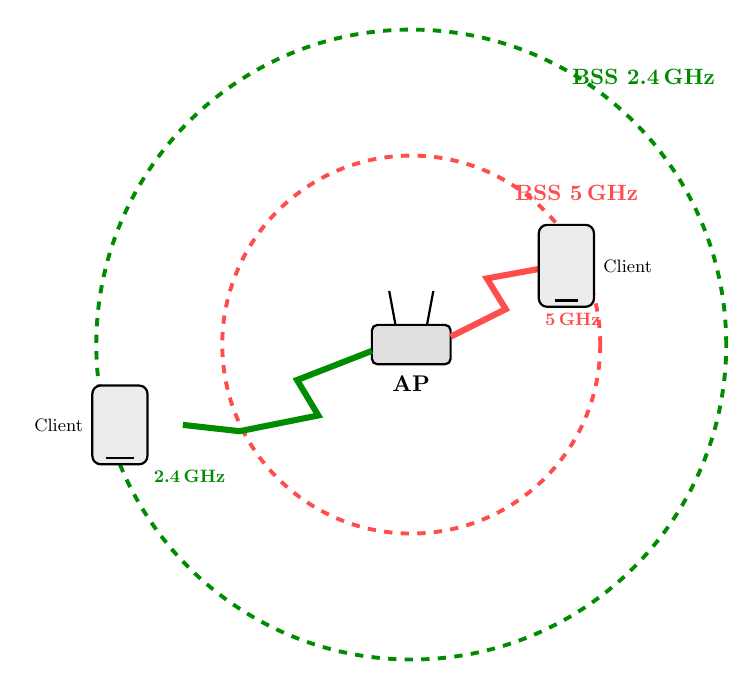
\begin{tikzpicture}[>=stealth, font=\small]
		
		% ---- Vùng phủ sóng ----
		% Ngoài: 2.4 GHz (xanh lá, dashed)
		\draw[green!55!black, dashed, line width=1.4pt] (0,0) circle (4.0cm);
		% Trong: 5 GHz (đỏ/hồng, dashed)
		\draw[red!60!pink, dashed, line width=1.4pt] (0,0) circle (2.4cm);
		
		% ---- Icon: AP (trung tâm) ----
		\draw[thick, fill=gray!25, rounded corners=2pt]
		(-0.50,-0.25) rectangle (0.50, 0.25);
		\draw[thick] (-0.20, 0.25) -- (-0.28, 0.68);
		\draw[thick] ( 0.20, 0.25) -- ( 0.28, 0.68);
		\node[below, scale=0.82, font=\bfseries] at (0,-0.30) {AP};
		
		% ---- Client gần: kết nối 5 GHz (bên phải, đỏ) ----
		% Lightning bolt AP → Client gần
		\draw[red!60!pink, line width=2.2pt]
		(0.50, 0.10) -- (1.20, 0.45) -- (0.96, 0.84) -- (1.62, 0.96);
		% Phone icon
		\draw[thick, rounded corners=3pt, fill=gray!15]
		(1.62, 0.48) rectangle (2.32, 1.52);
		\draw[thick] (1.82, 0.56) -- (2.12, 0.56);
		\node[right, scale=0.72] at (2.35, 1.00) {Client};
		\node[below right, scale=0.65, red!60!pink, font=\bfseries]
		at (1.62, 0.48) {5\,GHz};
		
		% ---- Client xa: kết nối 2.4 GHz (bên trái, xanh lá) ----
		% Lightning bolt AP → Client xa
		\draw[green!55!black, line width=2.2pt]
		(-0.50,-0.08) -- (-1.45,-0.45) -- (-1.18,-0.90) -- (-2.18,-1.10)
		-- (-2.90,-1.02);
		% Phone icon
		\draw[thick, rounded corners=3pt, fill=gray!15]
		(-4.05,-1.52) rectangle (-3.35,-0.52);
		\draw[thick] (-3.88,-1.44) -- (-3.52,-1.44);
		\node[left, scale=0.72] at (-4.08,-1.02) {Client};
		\node[below right, scale=0.65, green!55!black, font=\bfseries]
		at (-3.35,-1.52) {2.4\,GHz};
		
		% ---- Nhãn vùng phủ ----
		\node[green!55!black, scale=0.80, font=\bfseries] at ( 2.95, 3.40) {BSS 2.4\,GHz};
		\node[red!60!pink,    scale=0.80, font=\bfseries] at ( 2.10, 1.92) {BSS 5\,GHz};
		
	\end{tikzpicture}
	\caption{Mô hình chuyển băng tần (Band Steering) trên cùng AP.}
	\label{fig:BandSteering}
\end{figure}


\subsubsection{Chuyển vùng giữa các AP (Roaming)}

Đây là chức năng phân biệt mạng Mesh với các giải pháp mở rộng vùng phủ truyền thống.
Khi STA di chuyển khỏi vùng phủ tốt của AP hiện tại và tiến vào vùng phủ của AP khác,
hệ thống Mesh \textbf{chủ động gợi ý} STA chuyển vùng sang AP có kết nối tốt hơn ---
thay vì để STA tự bám víu vào AP cũ cho đến khi tín hiệu quá yếu.

Hai chuẩn 802.11 được sử dụng trong quá trình này:
\begin{itemize}
	\item \textbf{802.11k (Neighbor Report):} AP hiện tại cung cấp cho STA danh sách
	các AP lân cận và thông tin kênh của chúng, giúp STA quét mục tiêu nhanh hơn
	mà không cần quét toàn bộ phổ tần.
	\item \textbf{802.11v (BSS Transition Management):} AP gửi khung BTM Request gợi ý
	STA chuyển sang AP mục tiêu cụ thể. STA phản hồi chấp nhận hoặc từ chối;
	nếu từ chối và cần chuyển vùng bắt buộc, AP có thể dùng Disassociation.
\end{itemize}

Các ngưỡng RSSI, danh sách STA được phép/không được phép tự động chuyển vùng và chu
kỳ đo lường được cấu hình tập trung tại Controller thông qua \textbf{Steering Policy
	TLV} và phân phối đến tất cả Agent.

% ================================================================
% Hình 3: Roaming.png
% ================================================================
\begin{figure}[ht]
	\centering
	\begin{tikzpicture}[>=stealth, font=\small]
		
		% ---- Vùng phủ sóng (2 vòng tròn giao nhau) ----
		\draw[pink!80!red, dashed, line width=1.6pt] (-2.8, 0) circle (3.2cm);
		\draw[pink!80!red, dashed, line width=1.6pt] ( 2.8, 0) circle (3.2cm);
		
		% ---- Icon: AP 1 (trái) ----
		\draw[thick, fill=gray!25, rounded corners=2pt]
		(-3.35,-0.25) rectangle (-2.25, 0.25);
		\draw[thick] (-3.08, 0.25) -- (-3.18, 0.68);
		\draw[thick] (-2.52, 0.25) -- (-2.42, 0.68);
		\node[below, scale=0.78, font=\bfseries] at (-2.80,-0.30) {AP 1};
		
		% ---- Icon: AP 2 (phải) ----
		\draw[thick, fill=gray!25, rounded corners=2pt]
		(2.25,-0.25) rectangle (3.35, 0.25);
		\draw[thick] (2.52, 0.25) -- (2.42, 0.68);
		\draw[thick] (3.08, 0.25) -- (3.18, 0.68);
		\node[below, scale=0.78, font=\bfseries] at (2.80,-0.30) {AP 2};
		
		% ---- Client 1: đang kết nối AP 1 (trong vùng giao nhau) ----
		% Lightning bolt AP1 → Client1
		\draw[pink!80!red, line width=2.2pt]
		(-2.25,-0.12) -- (-1.38,-0.48) -- (-1.60,-0.90) -- (-0.75,-1.08);
		% Phone icon
		\draw[thick, rounded corners=3pt, fill=gray!15]
		(-0.75,-1.58) rectangle (-0.02,-0.55);
		\draw[thick] (-0.58,-1.50) -- (-0.22,-1.50);
		\node[below, scale=0.72] at (-0.38,-1.60) {Client};
		
		% ---- Client 2: đã chuyển sang AP 2 (bên phải) ----
		% Lightning bolt AP2 → Client2
		\draw[pink!80!red, line width=2.2pt]
		(3.35, 0.12) -- (4.18, 0.55) -- (3.95, 0.94) -- (4.80, 1.10);
		% Phone icon
		\draw[thick, rounded corners=3pt, fill=gray!15]
		(4.80, 0.62) rectangle (5.52, 1.65);
		\draw[thick] (4.98, 0.70) -- (5.30, 0.70);
		\node[right, scale=0.72] at (5.55, 1.12) {Client};
		
		% ---- Mũi tên chuyển vùng (cong, từ Client1 sang Client2) ----
		\draw[->, thick, dashed, blue!65]
		(-0.38,-0.55) .. controls (1.5, 1.2) and (3.0, 1.4) .. (4.80, 1.10);
		\node[blue!65, scale=0.74, font=\bfseries] at (2.2, 1.52)
		{Chuyển vùng (Roaming)};
		
	\end{tikzpicture}
	\caption{Mô hình chuyển vùng giữa các AP (Roaming) trong mạng Mesh.}
	\label{fig:Roaming}
\end{figure}

\begin{table}[ht]
	\centering
	\caption{Nội dung bản tin Link Metric Query trong IEEE~1905.1}
	\begin{tabular}{|>{\raggedright\arraybackslash}m{5cm}|>{\raggedright\arraybackslash}m{8cm}|}
		\hline
		\textbf{TLV} & \textbf{Mô tả} \\
		\hline
		AL MAC Address TLV & Địa chỉ AL MAC của thiết bị yêu cầu \\
		\hline
		Link Metric Query TLV & Chỉ định thiết bị đích cần truy vấn và loại metric yêu cầu: Transmitter, Receiver hoặc cả hai \\
		\hline
		Vendor Specific TLV (tùy chọn) & Mở rộng theo nhà sản xuất \\
		\hline
	\end{tabular}
\end{table}

\begin{table}[ht]
	\centering
	\caption{Nội dung bản tin Link Metric Response trong IEEE~1905.1}
	\begin{tabular}{|>{\raggedright\arraybackslash}m{5cm}|>{\raggedright\arraybackslash}m{8cm}|}
		\hline
		\textbf{TLV} & \textbf{Mô tả} \\
		\hline
		AL MAC Address TLV & Địa chỉ AL MAC của thiết bị phản hồi \\
		\hline
		Transmitter Link Metric TLV & Hiệu năng liên kết Tx: MAC đích, throughput ước tính, RSSI, tỉ lệ lỗi gói tin \\
		\hline
		Receiver Link Metric TLV & Hiệu năng liên kết Rx: các chỉ số tương tự từ phía nhận \\
		\hline
		Vendor Specific TLV (tùy chọn) & Chỉ số mở rộng: độ trễ, jitter, \ldots \\
		\hline
	\end{tabular}
\end{table}

\begin{table}[ht]
	\centering
	\caption{Nội dung bản tin AP Metrics Query / Response trong EasyMesh}
	\begin{tabular}{|>{\raggedright\arraybackslash}m{5cm}|>{\raggedright\arraybackslash}m{8cm}|}
		\hline
		\textbf{TLV} & \textbf{Mô tả} \\
		\hline
		AL MAC Address TLV & Địa chỉ AL MAC của thiết bị gửi \\
		\hline
		AP Metrics Query TLV & Controller yêu cầu dữ liệu hiệu năng của một hoặc nhiều BSS/Radio: MAC Agent, BSSID cụ thể, loại metric cần thu thập \\
		\hline
		AP Metrics Response TLV & Agent trả về: BSSID/Radio MAC, traffic uplink/downlink, channel utilization, error rate, retransmission count \\
		\hline
		Vendor Specific TLV (tùy chọn) & SNR, latency, jitter và các chỉ số bổ sung \\
		\hline
	\end{tabular}
\end{table}


% ============================================================
\section{Một Số Vấn Đề Thực Tế Cần Lưu Ý}
% ============================================================

Trong quá trình phát triển và vận hành hệ thống Wi-Fi Mesh, có bốn nhóm vấn đề thực
tế thường gặp cần được chú trọng:

\begin{enumerate}
	\item \textbf{Cấu hình chính xác vai trò BSS (fBSS / bBSS / bSTA):}
	Ba loại BSS này phải được cấu hình đúng vai trò xuống Driver Wi-Fi. Sai sót
	phổ biến nhất là cấu hình nhầm bSTA thành fBSS khiến Agent không thể thiết
	lập liên kết Backhaul, hoặc cấu hình bBSS trên Agent để phát sóng cho thiết
	bị người dùng thay vì chỉ dành cho bSTA. Những lỗi này thường khó phát hiện
	vì kết nối vật lý vẫn thành công nhưng đồng bộ cấu hình thất bại âm thầm.
	
	\item \textbf{Đồng bộ khi khởi động lại hoặc kết nối lại đồng loạt:}
	Khi nhiều Agent kết nối lại Controller cùng lúc (sau mất điện hoặc khởi động
	lại hệ thống), thuật toán xử lý bản tin đồng bộ phía Controller phải đủ khả
	năng phục vụ đồng thời nhiều phiên Autoconfig. Nếu phần mềm giữa Controller
	và Agent có phiên bản khác nhau với thuật toán đồng bộ không tương thích,
	một số Agent có thể không nhận được cấu hình hoặc nhận cấu hình sai ---
	trường hợp này xảy ra phổ biến khi mesh thiết bị xuyên thế hệ Wi-Fi~5/Wi-Fi~6.
	
	\item \textbf{Thuật toán chuyển vùng không đồng nhất giữa các phiên bản:}
	Phần mềm mới thường có thuật toán Steering cải tiến hơn phiên bản cũ. Tuy
	nhiên khi mạng bao gồm cả AP phiên bản cũ (đã triển khai đại trà chưa được
	cập nhật) và AP phiên bản mới, Controller và Agent có thể sử dụng các ngưỡng
	và logic chuyển vùng khác nhau --- dẫn đến STA bị ping-pong giữa các AP hoặc
	không được chuyển vùng kịp thời. Cần đặc biệt lưu ý khi AP phiên bản cũ
	đảm nhận vai trò Controller, vì thuật toán của Controller quyết định toàn bộ
	chính sách Steering cho mạng.
	
	\item \textbf{Ổn định của Driver Wi-Fi và Switch:}
	Toàn bộ hệ thống Mesh ở lớp ứng dụng hoạt động đúng theo thiết kế vẫn có
	thể gặp lỗi nếu Driver Wi-Fi hoặc Switch phần cứng không ổn định. Các biểu
	hiện thường gặp gồm: mất gói tin bất thường trên Backhaul, trễ cao đột ngột,
	hoặc interface Wi-Fi bị treo không phục hồi tự động. Nhà phát triển hệ thống
	Mesh cần nắm rõ giới hạn và lỗi đã biết của Driver để tránh nhầm lẫn lỗi
	phần cứng với lỗi phần mềm lớp trên.
\end{enumerate}